\chapter{Aufgabe 3}

\section{a)}

\textit{Entwurf des Dateisystems einschließlich einer Beschreibung der in den Dateien
gespeicherten Daten.}\\

\noindent
Es folgt eine grobe Beschreibung der Datei-Struktur der Anwendung, die in Abbildung~\ref{fig:struktur} und in Tabelle~\ref{tab:struktur} zusätzlich gelistet ist.
Die Nummerierung der Dateien (Subskripte) dient hierbei der Veranschaulichung :

\begin{itemize}
    \itemsep0.5em
    \item \textbf{DF - Dedicated Files}
    \begin{itemize}
        \item \textit{MF}: Wurzelverzeichnis der Chipkarte
        \item \textit{DF$_{\text{AID}}$}: Wurzelverzeichnis \underline{einer} Anwendung (vgl.~\cite[60]{ITS5}), beinhaltet PIN, Anwendungsdaten, systemweit bekannter Masterschlüssel der Anwendung (vgl.~\cite[46]{ITS5})
    \end{itemize}
    \item \textbf{EF - Elementary Files}
    \begin{itemize}
    \item  \textit{EF$_{\text{ICSSN}}$} (\textbf{Linear Fixed}): Dateityp fixer Länge zur Speicherung der \textit{Integrated Circuit Card Serial Number}, aus der ein Schlüssel abgeleitet wird.
    (Access-Mode \texttt{READ-ONLY})
    \item \textit{DF$_{\text{AID}}$.EF$_{\text{n}}$} (\textbf{Cyclic}): Da eine PIN-Eingabe erfolgt, muss die Anwendung auf der Chipkarte die Anzahl der Fehlversuche
    für eine mögliche Sperrung der Karte protokollieren.
    Hierfür wird der Befehl \texttt{INCREASE} / \texttt{DECREASE} genutzt,
    der nach ISO/IEC 7816 diesem Dateityp zur Verfügung steht (vgl.~\cite[45]{ITS5})
    \item \textit{DF$_{\text{AID}}$.EF$_{\text{PIN}}$} (\textbf{Linear Fixed}): Dateityp fixer Länge zur Speicherung der PIN (Access-Mode \texttt{READ-ONLY}).
    \item \textit{DF$_{\text{AID}}$.EF$_{\text{MK}}$} (\textbf{Linear Fixed}): Masterschlüssel einer Anwendung, der für die Berechnung des Schlüssels \textit{K$_{\text{AID}}$} genutzt wird (Access-Mode \texttt{READ-ONLY}).
        \end{itemize}
\end{itemize}


\begin{table}[h]
    \setlength{\tabcolsep}{0.5em}
    \def\arraystretch{1.5}
    \centering
    \begin{tabular}{|l|c|l|p{7cm}|}
        \hline
        \textbf{Datei} & \textbf{FID} & \textbf{Struktur} & \textbf{Beschreibung} \\
        \hline
        MF & $3F00$ & Top-Level Dedicated File & Wurzelverzeichnis der Chipkarte \\
        \hline
        EF$_{\text{ICSSN}}$ & $0001$ & Linear Fixed & ICSSN der Karte \\
        \hline
        DF$_{\text{AID}}$ & -- & Dedicated File & Verzeichnis einer Anwendung \\
        \hline
        D$_{\text{AID}}$.EF$_n$ & $\ldots$ & Cyclic & Protokollierung von Fehlversuchen bei PIN-Eingabe (Sperrzähler, \texttt{DECREASE}) \\
        \hline
        DF$_{\text{AID}}$.EF$_{\text{PIN}}$ & $\ldots$ & Linear Fixed & Speicherung der PIN \\
        \hline
        D$_{\text{AID}}$.EF$_{\text{MK}}$ & $\ldots$ & Linear Fixed & Speicherung des Masterschlüssels der Anwendung  \\
        \hline
    \end{tabular}
    \caption{Übersicht über die Dateistruktur der SSO-Chipkartenanwendung nach ISO/IEC 7816. Nicht angegeben sind die \textit{ARR}-Dateien (\textit{Access Rule Reference}) (Quelle: Struktur und Notation in Anlehnung an~\cite[\textbf{Tabelle 15.11}, 897]{RE02})}
    \label{tab:struktur}
\end{table}


\begin{figure}
    \centering
    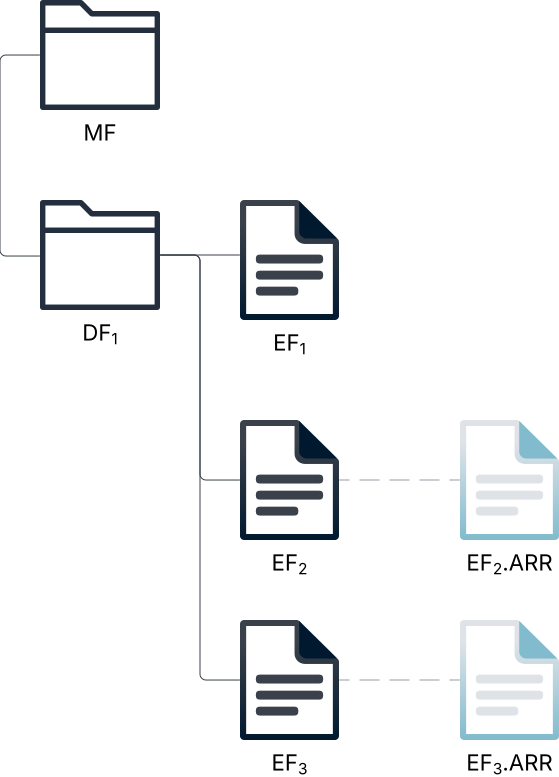
\includegraphics[scale=0.4]{aufgabe 3/img/struktur.svg}
    \caption{Skizze der Dateistruktur als Lösungsvorschlag für die in Aufgabe 3 beschriebene Chipkartenanwendung. (Quelle: eigene)}
    \label{fig:struktur}
\end{figure}

\section{b)}

\textit{Erstellen des Ablaufdiagramms einschließlich der Spezifikation der Chipkarten
kommandos, deren Parameter und einer Beschreibung des Ablaufs.}\\

\noindent
Das Ablaufdiagramm ist in Abbildung~\ref{fig:ablaufdiagramm} angegeben.
Wir stützen uns hierbei auf die Abbildungen~\cite[\textbf{Abb. 3.3 und 3.4}, 46 f.]{ITS5}, denen Details zu den verwendeten Verfahren \textbf{Mutual Authenticate} und \textbf{PIN-Verifikation} zu entnehmen sind: So wird in dem Ablaufdiagramm nicht explizit dargestellt, was bei erfolgloser PIN-Verifikation geschieht. Möglich wären - je nach erfüllter Bedingung -  eine Wiederholung der Eingabe, Sperrung Anwendung usw.


\noindent
Der grundsätzliche Ablauf stellt sich hierbei wie folgt dar:

\begin{enumerate}
    \itemsep0.5em
    \item Auswahl einer Anwendung
    \item Gegenseitige Authentifikation der Anwendung und der Chipkarte anhand des \textbf{Masterschlüssels} EF$_{\text{MK}}$ und der ICCSN E$_\text{ICSSN}$
    \item Eingabe der PIN
    \item Freischaltung der Anwendung bei Erfolg, sonst Sperre
\end{enumerate}

\noindent
Die Auswertung der Responses erfolgt - wie in den vorherigen Aufgaben bereits beschrieben - über die \textit{Statusbytes} \code{SW1} sowie \code{SW2} (s. Abbildung ~\ref{fig:rapdu}).


\begin{figure}
    \centering
    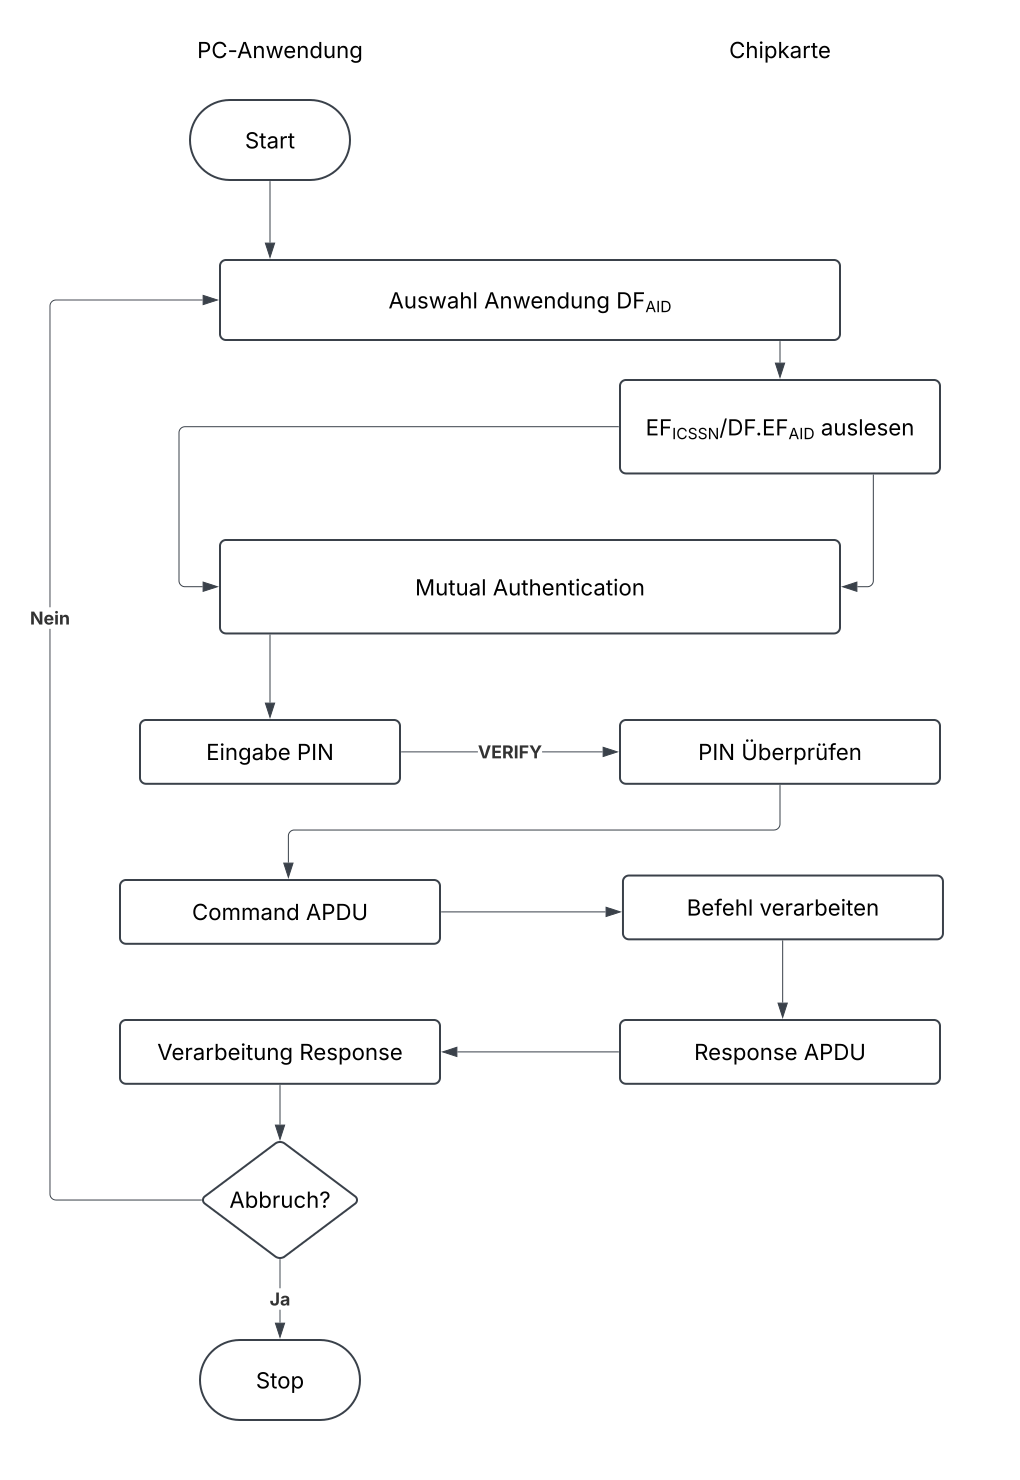
\includegraphics[scale=0.3]{aufgabe 3/img/ablaufdiagramm.svg}
    \caption{Ablaufdiagramm der Kommunikation zwischen PC und Anwendung bei einer SSO-Lösung. Es wurde versucht, die Aktionen so anzuordnen, dass sie die Verantwortlichkeiten der beteiligten Akteure widerspiegeln. (Quelle: eigene)}
    \label{fig:ablaufdiagramm}
\end{figure}